%************************************************
\chapter{Elección del Algoritmo}
\label{ch:algorithm}
%************************************************
\citeauthor{yamada2003} \cite{yamada2003} proponen un método para analizar las
dependencias palabra-a-palabra mediante una estrategia \emph{bottom-up} -- de
abajo a arriba. -- Para ello se hace uso de la técnica de \ac{AA}
\acfi{SVM}. Sus experimentos se basan en árboles de dependencias creados a
partir del corpus \ac{PTB}, logrando una precisión superior al 90\% para
dependencias palabra-a-palabra. Aún siendo esta precisión inferior al
\nameref{sec:stateoftheart}, hay que tener en cuenta que este método no utiliza
información sobre la estructura de las frases.

\begin{tikzpicture}[every node/.style={align=center},level distance=2cm]
\tikzset{edge from parent/.append style={<-}}
\Tree [.{said\\VBD} 
          [.{Inc.\\NNP}
             [.{Rolls-Royce\\NNP} ] [.{Motor\\NNP} ] [.{Cars\\NNPS} ] 
          ]
          [.{expects\\VBZ}
             [.{it\\PRP} ]
             [.{remain\\VB}
                [.{sales\\NNS}
                   [.{its\\PRP\$} ]
                   [.{U.S\\NNP} ]
                ]
                [.{to\\TO} ]
                [.{steady\\JJ} ]
                [.{at\\IN} [.{cars\\NNS} [.{about\\IN} [.{1200\\CD} ] ] ] ]
             ]
          ]
        ]
\end{tikzpicture}

%*****************************************
%*****************************************
%*****************************************
%*****************************************
%*****************************************
